%%% Local Variables: 
%%% mode: latex
%%% TeX-master: "../KanjiHWR"
%%% End: 

\chapter{Conceptual Design of Kanji-Coach}
\label{chap:conceptualdesignofKanjicoach}

\section{Requirements of a Kanji Teaching E-Learning Application}
\label{sec:concept:requirements}

\subsection{General Considerations}
\label{sec:concept:generalconsiderations}

In order to create a concept for a Kanji teaching application,
a number of different aspects need to be taken into consideration.
These aspects emerge from the academic background concerning the Japanese script,
pedagogical and didactic knowledge about teaching languages and general
conceptions of e-learning applications.

Many efforts in designing e-learning applications are focused around the
teacher's view on learning. For designing an e-learning application that
is useful to students, the students view needs be taken into 
account~\shortcite{Alexander2007}. 
\shortciteANP{Ivashin2009}~\citeyear{Ivashin2009} criticises the technical 
dominance in e-learning and e-teaching processes, as the conceptual software
designs are not always supporting the didactic purpose of the software.
Therefore, the user view should be taken into account when conceptually designing
an e-learning application.
The requirement of a \emph{user-focused design} follows directly from this view.

For on-line e-learning, it is a known that readers only scan the textual 
information displayed. Therefore it is not useful to provide a user with 
large blocks of text, but rather with smaller chunks that encourage 
skimming over~\shortcite{Hamid2001}. It can be expected that the fact
that an e-learning process happens on-line does not greatly affect the user 
behaviour. Therefore, the observations made for on-line e-learning can
probably be applied to offline desktop application based e-learning.
The requirement of \emph{keeping textual information short and concise} derives
from that observation.

If e-learning is considered as a learning method in higher education, 
\emph{blended learning} seems to be the most suitable form of e-learning.
Blended learning means combining classroom activities with e-learning 
methods~\shortcite{Hettinger2008,Kahiigi2008}. Language learning is not 
necessarily considered as higher education. In case of studying Japanese,
with its specific difficulties in language and the script, language learning
is taken to an intellectual level that is at least close to higher education.
Thus, an e-learning application for any aspect of the Japanese language 
should not have the ambition of possessing the capability 
to \emph{teach Japanese}. Japanese is a complex language with a complex script.
E-learning applications should aim at supporting a learner's 
classroom efforts of studying the language. The requirement of 
\emph{focusing on a specific language aspect} can be drawn from this reasoning.
The prototype system designed in this work does not aim at being a complete
e-learning system, but rather offers individual learning components from which 
a user can choose what type of learning and which component best supports his 
study.

\subsection{Conceptual Considerations for E-Learning of Kanji}
\label{sec:concept:conceptualconsiderationsforelearningofKanji}

An e-learning application for Kanji should be an e-learning application for
vocabulary at the same time. It is conceptually not useful to split those two 
learning tasks~\shortcite{Stahlmann2004}.
Learning Kanji and Hànzì is a visual task. Learners need to focus on many little
details concerning a character. For example, the character~\cjk{曜} contains 18 
strokes that are difficult to distinguish from each other in a regular script 
size of 11pt. It is those details that make it difficult for a learner to 
remember a character. Thus, it is important to direct and guide the learner's 
perception and comprehension of the characters towards a construct of Radicals, 
rather than a combination of a large number of strokes~\shortcite{Stahlmann2004}.
When attempting to split characters into conceptual sub units for the ease of
a learner, three different approaches lend themselves to this goal.

\textbf{Firstly}, splitting the characters into certain strokes. There are 26 
original strokes in the writing system and each shape in all the characters can 
be drawn with a combination of those strokes~\shortcite{Foljanty1984}.
This approach does not seem to ease the task of memorising the Kanji.
It may be fairly easy to memorise 26 strokes, but the fact that around 
2,000 Kanji necessary for reading Japanese consist of these strokes, does not
imply that memorising those becomes any less difficult.

\textbf{Secondly}, splitting the characters into graphemes. There are several 
shapes in use in the Japanese and Chinese writing system. There are 79 
graphemes in use~\shortcite{Hadamitzky1995}.
Using graphemes as a conceptual unit for a learner seems much more useful than
employing the strokes as a direct sub unit of the Kanji.
Memorising all the graphemes may help a learner to study the Kanji, because all 
sub shapes of the characters are known. However, graphemes do not necessarily 
bear a meaning. Seen from a perspective of perception and cognition, 
the coherence between the different parts of a Kanji would be purely visual.
That can help learners with an outstanding visual memory, but probably not
the majority with an average visual memory.

\textbf{Thirdly}, splitting the characters into Radicals. Radicals are the 
conceptual sub units of Kanji characters and they bear a meaning of their 
own. The number of Radicals is larger than the number of graphemes, but not all 
Radicals are in use and some graphemes are Radicals themselves at the same 
time~\shortcite{Hadamitzky1995}.
The Radicals do not only bear a meaning, but also have a function in character
formation (see section~\ref{sec:typologyoftheKanji} for typology of the Kanji).
In order for a learner to memorise the Kanji, it seems useful to grasp the 
concept of Kanji typology and therefore character formation.
Equipped with the rules of character formation and a number of Radicals the
brain can link different parts of a Kanji character with other parts and 
other characters. For example when studying phonograms, the majority of the
Kanji characters, knowledge about the pronunciation of the phonetic Radical
will help the learner.

Among those three possibilities it seems most suitable to use a combination of 
the second and the third. Conceptually, the characters will be split into 
Radicals, but the system must know about the concept of a grapheme, too.
Ideally, the system would have data that distinguishes both.

\subsection{Classification of a Kanji Teaching Application}
\label{sec:concept:classificationofaKanjiteachingapplication}
%xxx What follows from E-Learning aspects of the whole thing?
%classification as an e-learning application.
%what type of application is it?
%which learning paradigm is followed?

\subsubsection{Classification in an E-Learning Context}
\label{sec:concept:classificationinelearning}

Different types of e-learning systems have been discussed in 
section~\ref{sec:elearn:classification}. In the course of designing a prototype 
system, design choices need to be made.
The design choice for the prototype will be an offline e-learning system that 
runs on a desktop PC.
This design choice does not follow a conceptual requirement, in fact it ignores
\shortciteANP{Ivashin2009}'s~\citeyear{Ivashin2009} criticism of technical 
dominance in e-learning systems. The choice is a purely technical choice, 
yet, it is driven by a conceptual requirement.
The purpose of the e-learning environment is to test to what extend a handwriting
recognition engine can help studying the Kanji. In order to examine that 
research question, the handwriting recognition needs to be implemented and 
integrated with the e-learning system. 
Thus, the design choice for an offline system was inevitable in the sense that 
the technical limitations of on-line applications form an obstacle for pen 
input of characters and fast recognition procedures.

According to the definition given 
by~\shortciteANP{Richert2007}~\citeyear{Richert2007} the Kanji teacher 
prototype is a \emph{computer based training} (CBT) system, as it does not use 
the Internet for communication or a web server for storage. 
According to her research, another criterion for identifying offline systems 
is that they are offered for distribution on CD-ROM or floppy disk.
That criterion can be regarded as obsolete, as it refers to specific storage 
media. Even if a higher level of abstraction is used to describe the
criterion, it is still obsolete, since \emph{a passive storage medium} is not 
necessary to describe what the criterion actually tries to define.
The criteria concerning communication and data storage are useful to confine
different types of e-learning applications.
Additionally, \emph{installability} can be used as a criterion for offline 
e-learning systems. \emph{Installability} here refers to 
\emph{the possibility to install a software on a computer system}, 
not the \emph{ease of installation}, 
which is defined in ISO9126 as \emph{installability} as 
well~\shortcite{Chua2004}. The ISO9126 type of installability will not be taken 
into account during the software evaluation, because it would be outside the 
scope of the thesis.

\noindent The levels of interactivity as described in 
section~\ref{sec:elearn:interactivity}:
\begin{enumerate}
\item \textbf{View and absorb objects} 
\item \textbf{View and absorb multiple displays} 
\item \textbf{Varying the form of representation} 
\item \textbf{Changing the content of a component - parameter or data variation}
\item \textbf{Generating objects or the content of a representation} 
\item \textbf{Constructive and manipulative actions through situation-dependent feedback}
\end{enumerate}
The prototype designed in this work is aimed at a level higher than 
level~\emph{(\ref{elearn:class:changingcontent})~Changing the content of a 
component}. It is targeted between the 
levels~\emph{(\ref{elearn:class:generateobjects})~Generating objects or 
the content of a representation} 
and~\emph{(\ref{elearn:class:constructivemanipulative})~Constructive and 
manipulative actions through situation-dependent feedback}.
Concretely, a user can:
\begin{itemize}
 \item Change the ideal shape of a character by storing a new gold standard.
 \item Create new characters and their descriptions
 \item Receive situation-dependent feedback even on the newly created characters,
       due to the nature of the error recognition algorithm that evaluates
       mathematically the distance between a gold standard character and
       an input.
       Additionally, characters are analysed structurally, therefore new 
       characters added by the user will automatically be classified and arranged
       among the other characters in the database of the system.
\end{itemize}
Thus, based on the levels of interactivity~\shortcite{Richert2007},
it can be concluded that the prototype provides a very high level of 
interaction. The levels serve as an evaluation measurement for the quality of 
e-learning applications.

\subsubsection[Classification of Kanji Coach]
{Classification of Kanji Coach Among Kanji Teaching Applications}
\label{sec:concept:classificationofkanjicoach}

\emph{Kanji Coach} is an e-learning system for Kanji characters. Its unique
features are
\begin{itemize}
  \item The internal handwriting recognition engine
  \item The error recognition performed by the handwriting recognition module
\end{itemize}

The conceptual use of the handwriting recognition engine is dealt with in 
section~\ref{sec:concept:integrationofhwrintolearning}. The error handling 
concept is presented in section~\ref{sec:concept:handlingerrors}.

There are several e-learning systems that are centred around learning to read 
and write Japanese:
\begin{enumerate}
    \item \textbf{JWPce}:
          \url{http://www.physics.ucla.edu/~grosenth/jwpce.html} \\
          Special text processing editor for Japanese as a foreign language,
          including dictionaries.
    \item \textbf{JFC}:
          \url{http://www.physics.ucla.edu/~grosenth/jfc.html} \\
          Application for learning Kanji.
    \item \textbf{JapAlpha}:
          \url{http://members.aol.com/JapAlpha/private/japa10.htm } \\
          Application for learning the phonetic letters of Japanese.
    \item \textbf{Hiragana und Katakana online lernen}:
          \url{http://www.theiling.de/schrift/#kanatop} \\
          Web site for studying Hiragana and Katakana.
    \item \textbf{Moji}:
          \url{http://moji.mozdev.org/} \\
          Web browser extension for immediate dictionary lookup of Kanji.
    \item \textbf{KanjiQuick}:
          \url{http://www.kanji.de/} \\
          Dictionary for Kanji-German with a translation module and a text to 
          speech module.
    \item \textbf{Kanji Gold}:
          \url{http://web.uvic.ca/kanji-gold/} \\
          E-Learning application for studying Kanji.
    \item \textbf{KanjiGym Light}:
          \url{http://www.kanjigym.de/} \\
          E-Learning application for studying Kanji with the Heisig 
          system.\footnote{The Heisig system is a method for studying Kanji,
            discussed in section~\ref{sec:japanesedifficulties}.}
    \item \textbf{Tagaini vocabulary teacher}:
          \url{http://www.tagaini.net/} \\
          Vocabulary teacher for Japanese.
    \item \textbf{Online vocabulary teacher}:
          \url{http://www.vokabeltrainer-online.net/} \\
          General vocabulary teacher for several languages including Japanese.
    \item \textbf{Kanji Teacher of SZSB}:
          \url{http://szsbls3.szsb.uni-saarland.de/kanji/} \\
          Online e-learning application for studying Kanji.
    \item \textbf{Skritter}:
          \url{http://www.skritter.com} \\
          Online e-learning application for studying Kanji including a
          handwriting input.
\end{enumerate}
Among the various e-learning applications centred around Japanese there are 
three different types of applications.

\begin{enumerate}
  \item \textbf{Dictionaries}. In the dictionary type of applications it is 
        possible to look up a Kanji and receive a translation in a different
        language, mostly English, sometimes German. Among those JWPCE is
        the most developed in the sense that it provides a Radical lookup.
        A user can choose a number of Radicals in a matrix of Radicals
        and the dictionary finds appropriate characters.
  \item \textbf{Vocabulary teachers}. Vocabulary teaching applications provide 
        interfaces for word look-up and foreign word input with either
        Unicode input or Latin transcription of Japanese words.
  \item \textbf{Script teachers}. Script teaching applications are designed 
        as two different types. Multiple choice applications and handwriting 
        input.
        \begin{itemize}
          \item \textbf{Multiple choice}. The large majority of e-learning 
                applications teaching the Japanese script (either the two types
                of Kana or the Kanji) have to use multiple choice for character
                input. The reason for that is that modern 
                Input Method Editors (IME)
                allow for a Latin input of Japanese words and provide the
                Kanji for the user. If the application would prompt the user
                with a task like \emph{What Kanji is pronounced 'inu'?}
                the user would have to type 'I-N-U' in order to be presented
                with the character \cjk{犬} by the IME. In other words there is 
                no cognitive task for the user except reading Latin characters 
                from the screen and typing them on the computer keyboard.
                Since that does not help with the task of learning the Kanji,
                the only chance is multiple choice. The user is presented a set 
                of characters and is asked to click on the one that had been 
                asked for.
          \item \textbf{Handwriting input}. There are only two applications
                that use a handwriting input method in order to teach the Kanji.
                However, none of the applications performs a handwriting 
                recognition. Those two applications are \emph{Skritter} and 
                \emph{KanjiGym Light}.
         \end{itemize}
\end{enumerate}

\paragraph{Skritter} uses a kind of stroke-based similarity measure for 
individual strokes. When the system prompts the user for a specific character,
it allows only the next correct stroke of that character as user input. 
Concretely, the user can just try to write any stroke. If it is close enough to 
the next correct stroke, it will be morphed into an idealised picture of that 
stroke. If not, Skritter will show the correct stroke.
The system is clearly not a handwriting recognition system.

\noindent Figures:
\begin{itemize}
 \item 
 Figure~\ref{fig:skritter:noIncorrectInput} shows that Skritter does not allow
 any incorrect input by the user. If the user tries to input an incorrect stroke
 the correct stroke is shown on the screen. That feature avoids any learning 
 from one's own errors, because the correct stroke is always given.

 \item 
 Figure~\ref{fig:skritter:morphInputToCorrectStroke} shows the way Skritter 
 morphs a user input to the correct position. The stroke length is adapted to 
 fit the character. The user's error concerning the stroke length disappears 
immediately without any comment by the system. The system only comments incorrect
stroke direction.

 \item 
 Figure~\ref{fig:skritter:highToleranceForMorphing} shows the high tolerance that
 Skritter allows when morphing. The user input stroke has the 
 correct shape and the right  direction, but the euclidean distance of the 
 input stroke and the ideal stroke is large. Nevertheless Skritter accepts that 
 stroke as a correct input without a comment or feedback to the user.
\end{itemize}

\begin{figure}[htbp]
\begin{center}
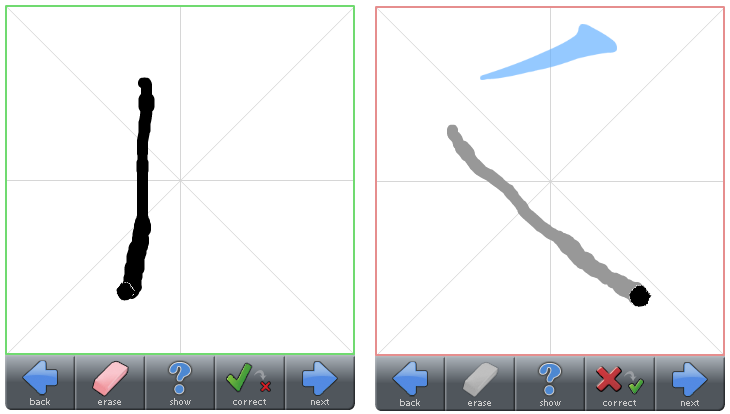
\includegraphics[scale=0.7]{images/ConceptualDesign/skritter/noIncorrectInput.png}
\caption{Skritter does not allow incorrect input}
\label{fig:skritter:noIncorrectInput}
\end{center}
\end{figure}

\begin{figure}[htbp]
\begin{center}
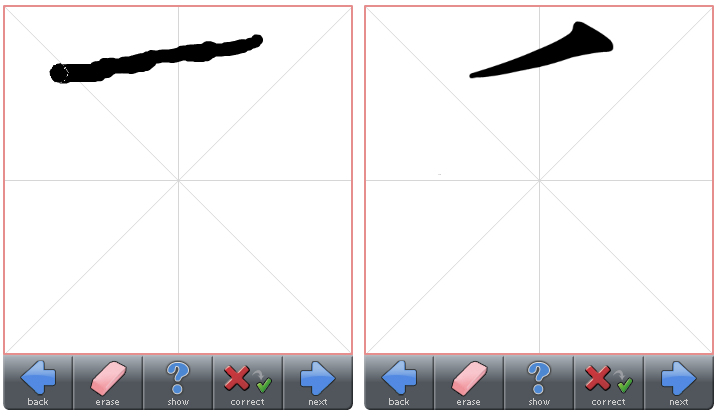
\includegraphics[scale=0.7]{images/ConceptualDesign/skritter/morphInputToCorrectStroke.png}
\caption{Skritter morphs user input to correct strokes}
\label{fig:skritter:morphInputToCorrectStroke}
\end{center}
\end{figure}

\begin{figure}[htbp]
\begin{center}
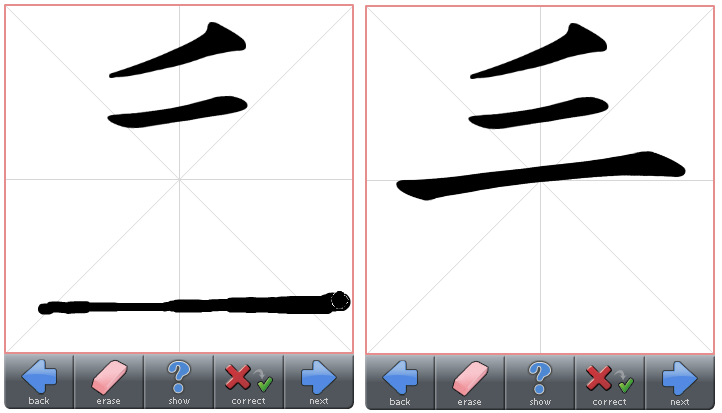
\includegraphics[scale=0.7]{images/ConceptualDesign/skritter/highToleranceForMorphing.png}
\caption{Skritter employs a very high tolerance when morphing user input}
\label{fig:skritter:highToleranceForMorphing}
\end{center}
\end{figure}

\paragraph{KanjiGym Light} does not perform a handwriting recognition. 
The application provides a canvas for writing characters. The user 
can input a character and then click a button named \emph{check}. The correct 
character appears next to the user input and leaves it to the user to compare 
for correctness. There is an accept and a discard button.
\begin{itemize}
\item Figure~\ref{fig:kanjigym:input} shows the user input canvas in 
      KanjiGym Light.
\item Figure~\ref{fig:kanjigym:check} shows the way KanjiGym Light has the 
      user compare his own input with the original character.
\end{itemize}

\begin{figure}[htbp]
\begin{center}
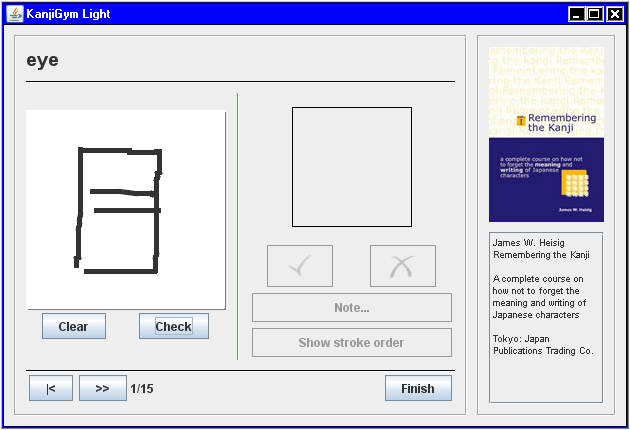
\includegraphics[scale=0.7]{images/ConceptualDesign/kanjigym/input.png}
\caption{KanjiGym Light character input}
\label{fig:kanjigym:input}
\end{center}
\end{figure}

\begin{figure}[htbp]
\begin{center}
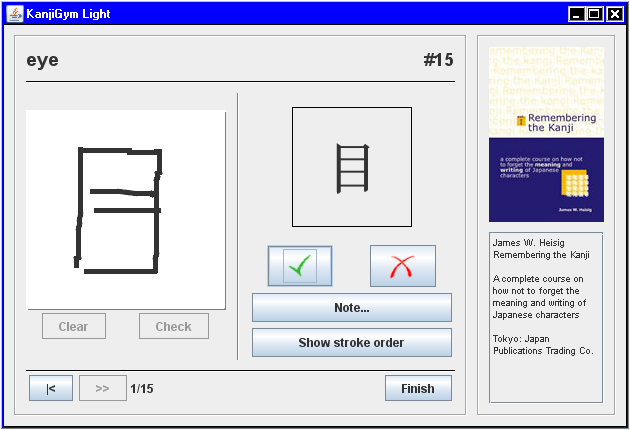
\includegraphics[scale=0.7]{images/ConceptualDesign/kanjigym/check.png}
\caption{KanjiGym Light checking correctness manually}
\label{fig:kanjigym:check}
\end{center}
\end{figure}

\section{Approaching the Specific Difficulties of the Japanese Script}
\label{sec:concept:tacklingdifficulties}

Section~\ref{sec:japanesedifficulties} deals with the typical problems that 
learners face when studying the Kanji. The Japanese script inevitably bears some 
difficulties when attempting to study it. The application should care for these 
problems by supporting these issues. They can be approached by providing
not only a handwriting input for the user but also a handwriting recognition
engine that gives informed feedback to the user.

\subsection{Character Learning Aspects}
\label{sec:concept:charaterlearningaspects}

The specific problems mentioned in section~\ref{sec:learnersproblems} are:
\begin{enumerate}
  \item \textbf{Similar Kanji} \label{enum:charlearning:similarKanji}
  \item \textbf{Compounds} \label{enum:charlearning:compounds}
  \item \textbf{Unusual readings} \label{enum:charlearning:unusualreadings}
  \item \textbf{Alternative Kanji} \label{enum:charlearning:alternativeKanji}
  \item \textbf{Homophones} \label{enum:charlearning:homophones}
  \item \textbf{Infrequent Jōyō Kanji} \label{enum:charlearning:infrequenjoyo}
  \item \textbf{Non-Jōyō Kanji} \label{enum:charlearning:nonjoyo}
\end{enumerate}

\subsubsection{Problems Outside the Scope of the Prototype}
\label{sec:concept:problemsoutsidescope}

A Kanji teaching prototype cannot provide solutions for all of those problems,
but for some. It cannot provide a satisfying solution for 
problem~\ref{enum:charlearning:compounds} as the prototype deals with single
characters only. It is not useful to provide a solution for 
problem~\ref{enum:charlearning:unusualreadings} because studying the main
reading of a character is most important at the beginning of studying Kanji. 
Especially, when studying a new character, the learner should focus on the 
character shape and the main reading, not on unusual alternative readings. 
Kanji Coach aims at teaching the Japanese script, not the full Japanese language.

Kanji Coach cannot provide a solution for 
problems~\ref{enum:charlearning:infrequenjoyo} 
and~\ref{enum:charlearning:nonjoyo}, memorising infrequent Jōyō 
Kanji and Non-Jōyō Kanji. These characters are difficult because they are 
infrequent. It seems more suitable for a learner to study the frequent characters
first in order to learn reading and writing. Thus, it is not plausible to pay 
special attention to this group of characters by presenting those more often to 
the learner.

\subsubsection{Problems Inside the Scope of the Prototype}
\label{sec:concept:problemsinscope}

The two main problems for learners of Japanese Kanji are 
\begin{itemize}
  \item Similar Kanji (problem~\ref{enum:charlearning:similarKanji})
  \item Homophones (problem~\ref{enum:charlearning:homophones})
\end{itemize}
Those two will be dealt with in the prototype. Additionally, the problem of
\begin{itemize}
  \item Alternative Kanji (problem~\ref{enum:charlearning:alternativeKanji})
\end{itemize}
is targeted by the e-learning application.

\paragraph{Similar Kanji} are the major issue for a learner of Japanese. The 
prototype \emph{Kanji Coach} provides a solution for this difficulty.
The solution does not necessarily contain the employment of specialised lessons 
for similar-looking Kanji. The reason for that is that it is more suitable for 
the human brain to study material that belongs to the same range of topics. 
Similar looking Kanji often do not have a connection to each other except their 
visual similarity. Therefore, studying them together does not seem useful,
unless they are semantically similar, too, like for instance the characters for
\emph{speaking} \cjk{話}, \emph{state/give instructions} \cjk{誥} and 
\emph{language} \cjk{語} that also belong to the same Kanji class, 
as their key Radical is the same.

\paragraph{Homophones} are a general difficulty for learners of the Japanese 
language. Many words are phonetically ambiguous. The context can provide a better
understanding, but often it is necessary to see the written Kanji character in 
order to know what is meant with an expression~\shortcite{Foljanty1984}.
Therefore, it is essential to deal with 
problem~\ref{enum:charlearning:homophones}. 

Conceptually, this issue can be solved by providing special lessons that focus on
homophones. Homophones in Japanese are not necessarily homographs and therefore 
not homonyms in the strict sense. True homonyms are those word pairs that are 
both homophones and homographs. In languages using Latin characters,
homophones are often homographs at the same time, e.g.\ German \emph{Schloss} 
(Eng.\ castle) and \emph{Schloss} (Eng.\ lock). This is due to the fact that
the spelling roughly mimics the speech. The pairs that are both homophones and
homographs are called homonyms. Sometimes, homophones are not homographs, 
e.g.\ the verbs \emph{dye} and \emph{die}.

In the course of studying the Kanji, it is part of the study process to 
learn to distinguish the characters that are pronounced the same.
For instance, there are roughly 80 distinct characters that share the
pronunciation \emph{kyo}. Table~\ref{table:kicombinations} on 
page~\pageref{table:kicombinations} shows several Kanji that are 
pronounced~\emph{ki}. The prototype provides a lesson that is centred around 
the homophone Kanji characters and their distinction.

\paragraph{Alternative Kanji} is an issue that can be dealt with in an indirect
way. Following the concept that frequent characters and the main reading should 
be studied first, Kanji Coach does not provide any special form of presentation
for this group of characters. However, it has the ability to recognise 
alternative Kanji. In a scenario where a user is asked to input a certain 
character, an alternative character with the same meaning would be accepted. 
For instance, if a user is prompted for the character for the number \emph{one}, 
which is usually written as~\cjk{一}, but enters the character~\cjk{壱} instead
this input would be regarded as correct. Additionally, the user is presented 
with a hint that another character with the same meaning exits. 
The focus lies on studying the frequent characters, therefore there are no 
special lessons concerning alternative Kanji.

\subsubsection{Character Repetition}
\label{sec:concept:characterrepetition} %label in use already.

In section~\ref{sec:elearn:elearningoflanguages} the pure repetition of 
grammatical structures as a learning method has been criticised.
The system should account for that by not just forcing the user to
reproduce fixed structures. In fact, it should leave room for creativity.
The system does not provide a free-drawing module in order to allow for
total creativity. But creativity is given through the use of the
handwriting input as such. A user can practise his own writing style.
The tolerance thresholds given by the character recognition module allow for an
interpretation of the character shape, rather than a pure repetition.

Similar to the multi-radical look-up in JWPCE a learning task for a user
of the Kanji e-learning prototype \emph{Kanji Coach} could be the combination 
of different radicals to a Kanji character.
That would allow for creativity and also appeal to the cognition because
it is more demanding than merely repeating the shapes that were given before.

%Zum Beispiel - radikale vorgeben und zeichen schreiben lassen.
%und ganz generell: toleranzgrenzen erlauben kreativitaet allein schon deswegen,
%weil selbst der zeichenstift benutzt wird.

\section{Integration of HWR Into the Learning Process}
\label{sec:concept:integrationofhwrintolearning}

The learning process of Kanji is driven by understanding the structure and 
meaning of the characters and memorising the shape~\shortcite{Stahlmann2004}. 
In order to study and memorise, many learners rely on repeating to write the 
Kanji. That approach seems most natural and can hardly be replaced by any other 
method. Nevertheless, the method can be changed to be more challenging to
a user and thus create some level of excitement. This is done by combining
it with different tasks where the user does not see the character before
having to write it.

\subsection{The Motivation for Using a HWR}
\label{sec:concept:motivationforusinghwr}

The fact that learning to read and learning to write are highly interwoven 
processes suggests that both should be studied together. In standard class room 
learning environments that is the case. Learners read texts, learners are 
presented with new Kanji and learners are asked to reproduce the Kanji when 
writing essays.
An e-learning application can not perform the teaching effort of a full language
course. In order to provide a complementary addition to a language course,
the prototype should create an environment that increases the user's regalement 
for tedious learning tasks.

The repetition of writing characters in order to memorise them does not
appeal to the majority of the learners. Especially having to write on paper
repeating the same character over and over again does not awake inspiration
and creativity. An e-learning application with an integrated handwriting 
recognition engine that provides corrections for the user input has two 
main functions:
\begin{itemize}
  \item Making the repetitive task of training the muscular memory less tedious.
  \item Helping the learner overcome difficulties in writing the Kanji by 
        giving informed feedback.
\end{itemize}
In order to train the muscular memory and memorise the Kanji, repetition is 
needed. The same amount of written characters can seem less repeating simply if
the characters are not written in a row. Additionally, using a technical device 
can be more emotive and help increasing the user's motivation and 
self-discipline. \shortcite{Ismail2002,Richert2007} criticised that some 
e-learning applications do not add a value to the learning 
process.\footnote{For details see section~\ref{sec:elearn:elearningoflanguages}.}
The prototype proposed in this work does add value to the learning process.
Additional value over practising to write characters on paper is added
by the following features:
\begin{itemize}
  \item The general ability of the application to prompt the user with 
        different characters in an ordered or random fashion.
  \item Presentation new characters, their meanings, pronunciation and
        stroke order.
  \item Characters are organised in lessons and related characters are presented
        in combination with each other in the same lesson.
  \item The methods
    \begin{itemize}
      \item Writing a Japanese character after being prompted an English word, 
            instead of purely drawing lines without an additional cognitive 
            anchor.
      \item Writing a Japanese character after being prompted a Japanese word.
    \end{itemize}
  \item The error correction that comes with the handwriting recognition. The 
        user is less dependent on a teacher and can study in his own time and 
        pace, yet still get informed feedback.
\end{itemize}
 
\subsection{Character Recognition}
\label{sec:concept:characterrecognition}

The type of character recognition is crucial for the abilities of the system 
concerning error processing. Highly optimised handwriting recognition systems
perform a fast and reliable handwriting recognition. However, those systems
often do not have a  record of the internal structure of the 
characters.\footnote{See chapter~\ref{chap:onlinehwr} for details.}
Since understanding of the structure of the characters is important for a 
successful learning process, the error correction needs to focus on the internal
structure of the Kanji characters. Studying the character shapes can be 
performed as a purely visual task. Studying the full characters and grasping
their construction is a cognitive task that combines visual memory with
linguistic information. Thus, the error correction must provide structural
error levels, considering the internal character structure. Following that
concept even further, the character analysis must be structural as well.
The prototype performs a structural character 
recognition.\footnote{Details about how the character recognition is
performed on a technical level can be found in 
chapter~\ref{chap:handwritingrecognitionengine}.}
Structural character recognition means that it performs a structural analysis
of the characters in order to obtain a symbolic value for the character,
in this case a unicode value. 

%xxx How do the HWR and the learning process interplay conceptually?
%xxx In what form do the corrections come up?
%xxx What kind of error recognition is there?
%xxx character input: timeout for learning - no button in handwriting data input view

% Wichtige Fragestellung: Wie sieht eine HWR in Lernumgebung aus?
% Mappe S. 19
% genaue anforderungen s. 19!
% waehle bestimmte architekture unter moeglichen ansaetzen.


% welche art von character recognition muss geleistet werden?

% was sind die moeglichkeiten (im vergleich zu anderen produkten),
% die sich durch eine HWR ergeben?
% wie kann man die ausschoepfen? s. 16 unten und s. 15

% Error Recognition
% what type of errors?
% semantical errors? cow vs.\ sheep vs.\ pig
% phonological errors (readings) Kanji that sound the same.
% theoretically: compounds - for the Kanji readings.
% heft: s. 52

% - compare with normal paper-based learning of Kanji
% - compare with other Kanji-learning systems
% klare abgrenzung von skritter.
% s. 51 unten im heft.


\section{Handling Errors}
\label{sec:concept:handlingerrors}

Having a handwriting recognition that gives informed feedback about the 
question if the entered character was correct is an approach that allows
for additional analysis and feedback.
Because of the structural analysis of the characters during the recognition 
process it becomes possible to provide feedback about errors on a graphemic, 
phonetic and semantic level.

%xxx why this section? what is its purpose?
%because it is one of the crucial novelties of the system to provide an
%error handling like this, therefore it must be reported.

%what is in this section:
%how to deal with errors conceptually
%what types of errors are there and how they can be handled
%outcome visioning: educational aspects / the e-learning view
%how? how will it be structured?
%next action - what to write first?

\subsection{Motivation for Error Recognition}
\label{sec:concept:motivationforerrorrecognition}

The motivation for error recognition has been broached in the previous sections.
The main reason is that a user needs be given a chance to learn from his own 
errors. In any relation between a student and a teacher, concerning any subject 
matter the teacher has the task to inform the student about mistakes.
The teacher provides corrections to the errors of the student when trying
to fulfil a task. The student can learn by improving what he had done wrong 
before. 

For an e-learning application it is difficult to provide an informed error 
correction. The reasons for that lie in:
\begin{itemize}
  \item The limitations of communication between the machine and the user:
        in the most common scenario the user interaction is limited to
        typing with the keyboard and clicking with the mouse
  \item The limitations of user input analysis. For text strings most of the
        times only exact matches are accepted. Some types of analyses are very
        difficult to perform, including syntax analysis and handwriting input.
        That is the reason for most interfaces to perform a simplified
        or a partial analysis of the user input or no analysis at all.
  \item Limited knowledge within the application about potential user errors.
\end{itemize}
In Kanji Coach these limitations shall be weakened. The communication between
machine and user is actualised with an intelligent user interface, a canvas that
takes handwritten characters as input. The limited user input analysis is
approached with the interpretation of the strokes as a Kanji character.
Knowledge about possible sources of error is stored in the application's 
knowledge base, such that the third limitation has a less severe impact into
user experience.

\subsection[Sources of Error]{Possible Sources of Error When Writing Japanese Characters}
\label{sec:concept:sourcesoferror}

There are seven different sources of errors for learners when writing Kanji 
characters. These error categories are:
\begin{itemize}
\item Stroke level errors
\item Radical level errors
\item Character level errors
\item Linguistic level errors
  \begin{itemize}
  \item Phonological errors
  \item Morphological errors
  \item Semantic errors
  \item Lexical errors
  \end{itemize}
\end{itemize}

\paragraph{Stroke level errors} 
\begin{itemize}
\item \textbf{Stroke length}: A stroke has been drawn by the user with an 
      incorrect length.
\item \textbf{Stroke direction}: The stroke has been drawn from the opposite
      direction or the general stroke direction, the absolute angle with respect 
      to the X-axis was deviant.
\item \textbf{Stroke angle}: If the stroke has a corner the angle of in the
      corner can deviate from the angle of the original stroke.
\end{itemize}

\paragraph{Radical level errors}
\begin{itemize}
\item \textbf{Stroke number}: The number of strokes in the Radical is different
      from the number of strokes in the gold standard Radical.
\item \textbf{Stroke sequence}: The sequence of strokes within the Radical
      is different from the ideal stroke sequence.
\end{itemize}

\paragraph{Character level errors}
\begin{itemize}
\item \textbf{Incorrect Radical}: A Radical used within the character is not
      correct as it was confused with a different one by the user.
\item \textbf{Incorrect number of Radicals}: An additional Radical has been 
      added to the character or a Radical is missing.
\end{itemize}

\paragraph{Linguistic level errors} are a super-category of other error category.
The errors on a linguistic level do not concern the character input directly
but rather the language and the use of the characters. The linguistic errors
can be subdivided into phonological, morphological, semantic and lexical errors,
where the latter ones have only a subtle distinction.

\paragraph{Phonological errors} are errors concerning Kanji readings. If a user
writes a character with the same reading as the character in question it is 
likely to be a confusion based on the phonological features of the two 
characters. The Japanese language has a large number of homophones that abet
this type of confusion.

\paragraph{Morphological errors} are mainly concerned with suffixation.
If a Kanji character and additional Hiragana characters in order to form a word,
these Hiragana characters are called \emph{Okurigana}.\footnote{For a detailed 
description of what Okurigana are, see 
section~\ref{sec:structureofwritingsystem}.}
The error of adding incorrect Okurigana to a Kanji character can be classified
as a morphological error. As the Kanji Coach prototype deals with single 
characters only this error type is not applicable.

\paragraph{Semantic errors} are those errors where a user confuses two characters
with a similar meaning. For example, the words 
\cjk{食べ物}~(Jap.~pron.~\cjk{タベモノ}~/~tabemono; 
Eng.~lit.~\emph{thing for eating}; Eng.~\emph{food}) 
and 
\cjk{飲み物}~(Jap.~pron.~\cjk{ノミモノ}~/~nomimono; 
Eng.~lit.~\emph{thing for drinking}; Eng.~\emph{drink})
can be confused easily on a semantic level. The same is true for the individual 
characters.
 
\paragraph{Lexical errors} are the errors where a user uses a character with the
same meaning. Those are not real errors. This falls under 
\emph{alternative Kanji} that have been discussed in 
section~\ref{sec:concept:problemsinscope}.
This type of error can be compared to using a synonym in a vocabulary test.
The word was not the word asked but the answer is not incorrect either.
Therefore, lexical errors do not need special attention the the prototype
application.

\section{Use Cases}
\label{sec:concept:usecases}

The uses cases presented in this section are oriented towards the conceptual
design presented in the previous chapters. The startup screen of the application
is presented in figure~\ref{fig:startupScreen}. There are four different modes 
to choose from.
\begin{enumerate}
\item View mode
\item Follow mode
\item Exercise mode 1
\item Exercises mode 2
\end{enumerate}
The user can employ different modes for self-directed study. In view mode,
the characters and information about those are just presented to the user.

Figure~\ref{fig:viewMode} shows the view mode. On the left side of the screen
the character is presented to the user. On the right side of the screen
information about the character are displayed.

The first interactive character learning mode is the follow mode shown in
figure~\ref{fig:followMode}. In follow mode, a character is shown and the user
can follow the character lines that are shown on the screen. 

The input in follow mode or in the other modes can be drawn on the mobile input
area. That guarantees the ability to use a stylus. 
Figure~\ref{fig:mobileDeviceInput} shows a drawing on the mobile device.
In exercise~mode~1 the user is presented an English word and is asked 
to draw the appropriate Kanji character. Exercise~mode~2 works the same way,
just the user is presented the Japanese reading of a character instead of the
English word.

Figure~\ref{fig:exerciseMode1} shows the screen of exercise~mode~1 with a
user input. The user input is mirrored from the mobile device as shown in 
figure~\ref{fig:mobileDeviceInput} before.
After the character recognition and error detection is performed,
the application can return an analysis to the user.
In this case the input was not quite correct. As seen in 
figure~\ref{fig:followMode} in order to write the character for 'root',
which is written \cjk{本}, there is one stroke missing in 
figure~\ref{fig:mobileDeviceInput} and the mirrored image in
figure~\ref{fig:exerciseMode1}.

\emph{Incorrect stroke number} is one of the errors defined in 
section~\ref{sec:concept:sourcesoferror}. It is in the 
\emph{Radical error level} as there is a stroke missing in order to
finish the Radical.
There is no error in character level. In this special case the character
is a Radical. The error 'missing stroke' is relevant to the Radical level.

Figure~\ref{fig:exerciseMode1Errormessage} shows the error message and
the feedback for the user. A missing stroke is just a minor error,
therefore the user is presented a positive feedback.

\begin{figure}[htbp]
\begin{center}
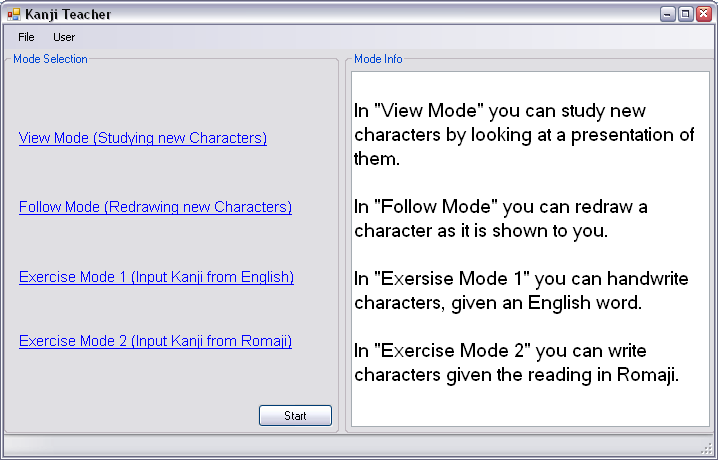
\includegraphics[scale=0.7]{images/ConceptualDesign/startupScreen.png}
\caption{Startup screen}
\label{fig:startupScreen}
\end{center}
\end{figure}

\begin{figure}[htbp]
\begin{center}
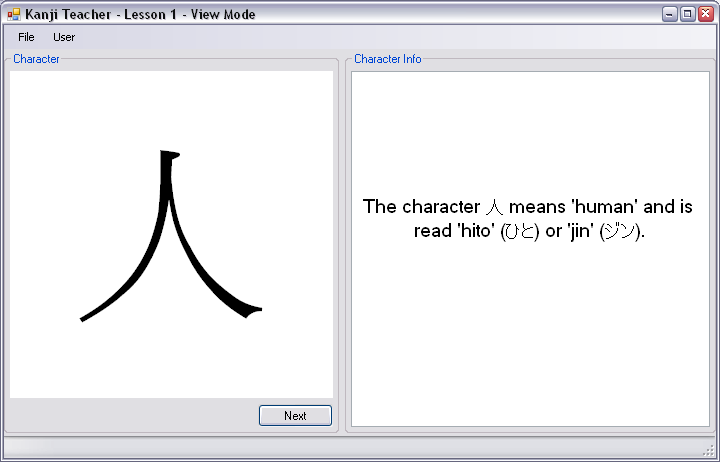
\includegraphics[scale=0.7]{images/ConceptualDesign/viewMode.png}
\caption{Character view mode}
\label{fig:viewMode}
\end{center}
\end{figure}

\begin{figure}[htbp]
\begin{center}
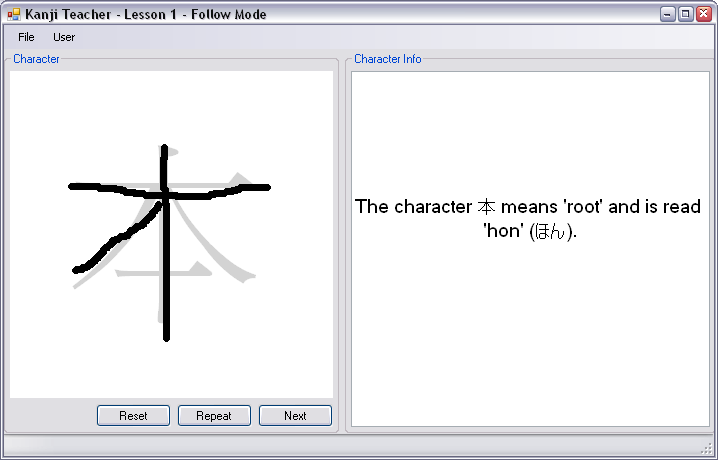
\includegraphics[scale=0.7]{images/ConceptualDesign/followMode.png}
\caption{Follow mode for drawing new characters}
\label{fig:followMode}
\end{center}
\end{figure}


\begin{figure}[htbp]
\begin{center}
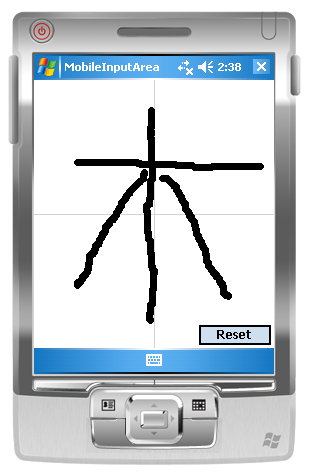
\includegraphics[scale=0.6]{images/ConceptualDesign/mobileDeviceInput.png}
\caption{Mobile device character input}
\label{fig:mobileDeviceInput}
\end{center}
\end{figure}

\begin{figure}[htbp]
\begin{center}
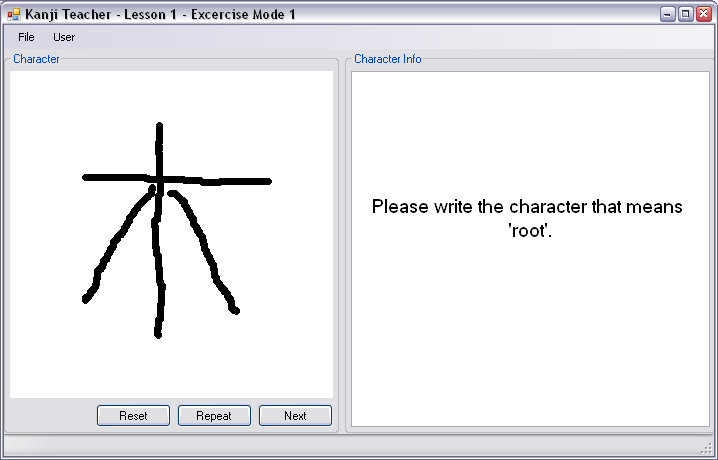
\includegraphics[scale=0.7]{images/ConceptualDesign/exerciseMode1.png}
\caption{Exercise mode 1 for input of Kanji from English source}
\label{fig:exerciseMode1}
\end{center}
\end{figure}

\begin{figure}[htbp]
\begin{center}
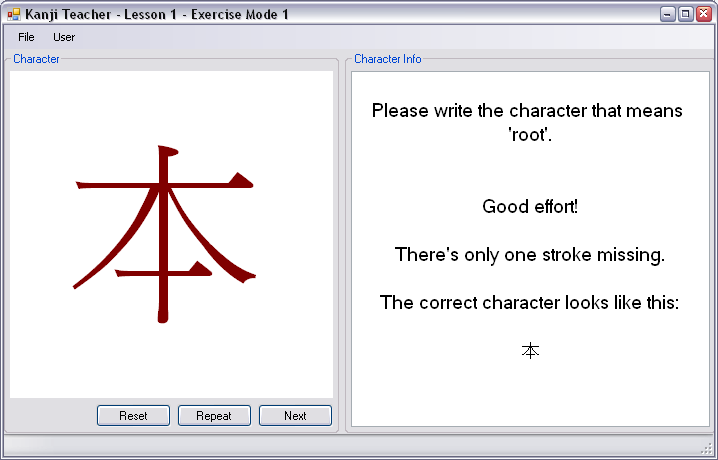
\includegraphics[scale=0.7]{images/ConceptualDesign/exerciseMode1Errormessage.png}
\caption{Exercise mode 1 after user entered almost correct character}
\label{fig:exerciseMode1Errormessage}
\end{center}
\end{figure}

% siehe 'screenshot' - grafiken von s. 2 - 9
% auch: was kann man aus e-learning machen?
% welche (technischen) moeglichkeiten sind eroeffnet,
% insbesondere auch durch handschriftenerkennung?

% idee: schoenschreibekurs, bei dem einzelne striche
% gesondert geuebt werden.

